\documentclass[conference]{IEEEtran}
\IEEEoverridecommandlockouts
% The preceding line is only needed to identify funding in the first footnote. If that is unneeded, please comment it out.
\usepackage{cite}
\usepackage{amsmath,amssymb,amsfonts}
\usepackage{algpseudocode}
\usepackage{algorithm}
\usepackage{graphicx}
\usepackage{textcomp}
\usepackage{xcolor}
\def\BibTeX{{\rm B\kern-.05em{\sc i\kern-.025em b}\kern-.08em
    T\kern-.1667em\lower.7ex\hbox{E}\kern-.125emX}}
\begin{document}

\title{SALCA-IB: Self-Adaptive LLM-Driven Continuous Learning Agent for IB Network Failure Prediction\\
{\footnotesize \textsuperscript{*}Note: Sub-titles are not captured in Xplore and
should not be used}
\thanks{Identify applicable funding agency here. If none, delete this.}
}

\author{\IEEEauthorblockN{1\textsuperscript{st} Given Name Surname}
\IEEEauthorblockA{\textit{dept. name of organization (of Aff.)} \\
\textit{name of organization (of Aff.)}\\
City, Country \\
email address or ORCID}
\and
\IEEEauthorblockN{2\textsuperscript{nd} Given Name Surname}
\IEEEauthorblockA{\textit{dept. name of organization (of Aff.)} \\
\textit{name of organization (of Aff.)}\\
City, Country \\
email address or ORCID}
\and
\IEEEauthorblockN{3\textsuperscript{rd} Given Name Surname}
\IEEEauthorblockA{\textit{dept. name of organization (of Aff.)} \\
\textit{name of organization (of Aff.)}\\
City, Country \\
email address or ORCID}
\and
\IEEEauthorblockN{4\textsuperscript{th} Given Name Surname}
\IEEEauthorblockA{\textit{dept. name of organization (of Aff.)} \\
\textit{name of organization (of Aff.)}\\
City, Country \\
email address or ORCID}
\and
\IEEEauthorblockN{5\textsuperscript{th} Given Name Surname}
\IEEEauthorblockA{\textit{dept. name of organization (of Aff.)} \\
\textit{name of organization (of Aff.)}\\
City, Country \\
email address or ORCID}
\and
\IEEEauthorblockN{6\textsuperscript{th} Given Name Surname}
\IEEEauthorblockA{\textit{dept. name of organization (of Aff.)} \\
\textit{name of organization (of Aff.)}\\
City, Country \\
email address or ORCID}
}

\maketitle

\begin{abstract}
InfiniBand Network (IB Network) failure prediction is crucial in high-performance computing and data center operations, yet faces significant challenges due to environmental complexity and dynamicity, such as scarcity of failure data and susceptibility of network feature distributions to external factors. This paper introduces \textbf{SALCA-IB} (Self-Adaptive LLM-Driven Continuous Learning Agent for IB Network Failure Prediction), an innovative adaptive failure prediction agentic system. SALCA-IB utilizes a Large Language Model (LLM) as its planning core, combined with traditional machine learning methods, to achieve autonomous prediction and optimization. The system's main innovations include: (1) LLM-driven autonomous data selection and model optimization; (2) A fusion memory system integrating short-term and long-term memory; and (3) LLM-supported automatic evaluation feedback and closed-loop optimization. Experimental results show that compared to traditional methods, SALCA-IB improves prediction accuracy by X\% and demonstrates a Y-fold increase when facing changes in network feature distributions. Our code is available at XXXX.github.com.
\end{abstract}

\begin{IEEEkeywords}
IB Network, Large Language Model, Autonomous Agent, Memory System
\end{IEEEkeywords}

\section{Introduction}
High-performance computing and modern data centers heavily rely on InfiniBand (IB) networks for their superior performance in low-latency, high-bandwidth communication. As the backbone of these critical infrastructures, IB networks' reliability directly impacts the overall system performance and service availability. However, network failures can lead to severe service disruptions and significant performance degradation, making failure prediction increasingly crucial for maintaining system reliability and operational efficiency.

Despite its importance, IB network failure prediction faces several significant challenges. First, failure data in IB networks is inherently scarce, as failures are relatively rare events, making it difficult to build robust prediction models using traditional machine learning approaches. Second, network feature distributions are highly dynamic and susceptible to various external factors, such as environmental conditions, hardware aging, and maintenance activities. Third, existing prediction systems often lack the ability to adapt to these changing conditions, resulting in degraded performance over time.

Traditional approaches to network failure prediction primarily rely on static machine learning models or rule-based systems (ADD REF). While these methods have shown some success in controlled environments, they struggle to maintain performance in real-world scenarios where network characteristics evolve continuously (ADD REF). Moreover, existing solutions often operate as black boxes, providing limited interpretability and failing to leverage historical experience effectively for continuous improvement.
 
The emergence of Large Language Models (LLMs) presents new opportunities for addressing these challenges. LLMs have demonstrated remarkable capabilities in complex reasoning and planning tasks (ADD REF) , suggesting their potential for orchestrating adaptive prediction systems. Additionally, recent advances in memory systems and continuous learning architectures (ADD REF) have shown promise in handling dynamic environments, though their application to network failure prediction remains largely unexplored.

To address these challenges, we propose SALCA-IB (Self-Adaptive LLM-Driven Continuous Learning Agent for IB Network Failure Prediction), an innovative system that combines the reasoning and planning capabilities of LLMs with traditional machine learning models in a unified, adaptive framework. SALCA-IB introduces several key innovations that directly address the aforementioned challenges: 
(1) To tackle the data scarcity issue, we develop an LLM-driven planning core that intelligently selects and utilizes limited training data, while orchestrating multiple lightweight models to maximize the value of available data;
(2) To handle dynamic feature distributions, we design a dual-memory system that integrates both short-term and long-term experiences, enabling the system to capture and adapt to evolving network characteristics while maintaining historical knowledge;
(3) To overcome the limitations of static prediction systems, we implement a continuous learning mechanism that enables real-time model updates and performance optimization, ensuring sustained prediction accuracy even as network conditions change.

Experimental results demonstrate that SALCA-IB outperforms traditional methods in terms of prediction accuracy and adaptability, achieving X\% higher accuracy and Y-fold improvement in prediction performance when facing network feature distribution changes. Ablation studies further confirm the significant contributions of both the LLM-driven planning and dual-memory system components.

To conclude, the main contributions of this paper are threefold:
\begin{itemize}
	\item We propose an innovative LLM-driven agent architecture (SALCA-IB) for IB network failure prediction. The system uniquely leverages LLM as a high-level planning core to orchestrate model selection, parameter optimization, and continuous learning strategies, while employing traditional machine learning models as efficient executors for real-time prediction tasks.
	\item We design a novel dual-memory fusion system that seamlessly integrates short-term and long-term memory mechanisms. This sophisticated memory architecture enables rapid adaptation to dynamic network changes while preserving and leveraging valuable historical knowledge, significantly enhancing the system's robustness and adaptability.
	\item We conduct comprehensive experiments on real-world IB network datasets to rigorously validate SALCA-IB's effectiveness. Through extensive ablation studies and comparative analyses, we demonstrate the substantial contributions of both the LLM-driven framework and the dual-memory system components to the overall system performance.
\end{itemize}

\begin{figure*}[htbp]
    \centering
    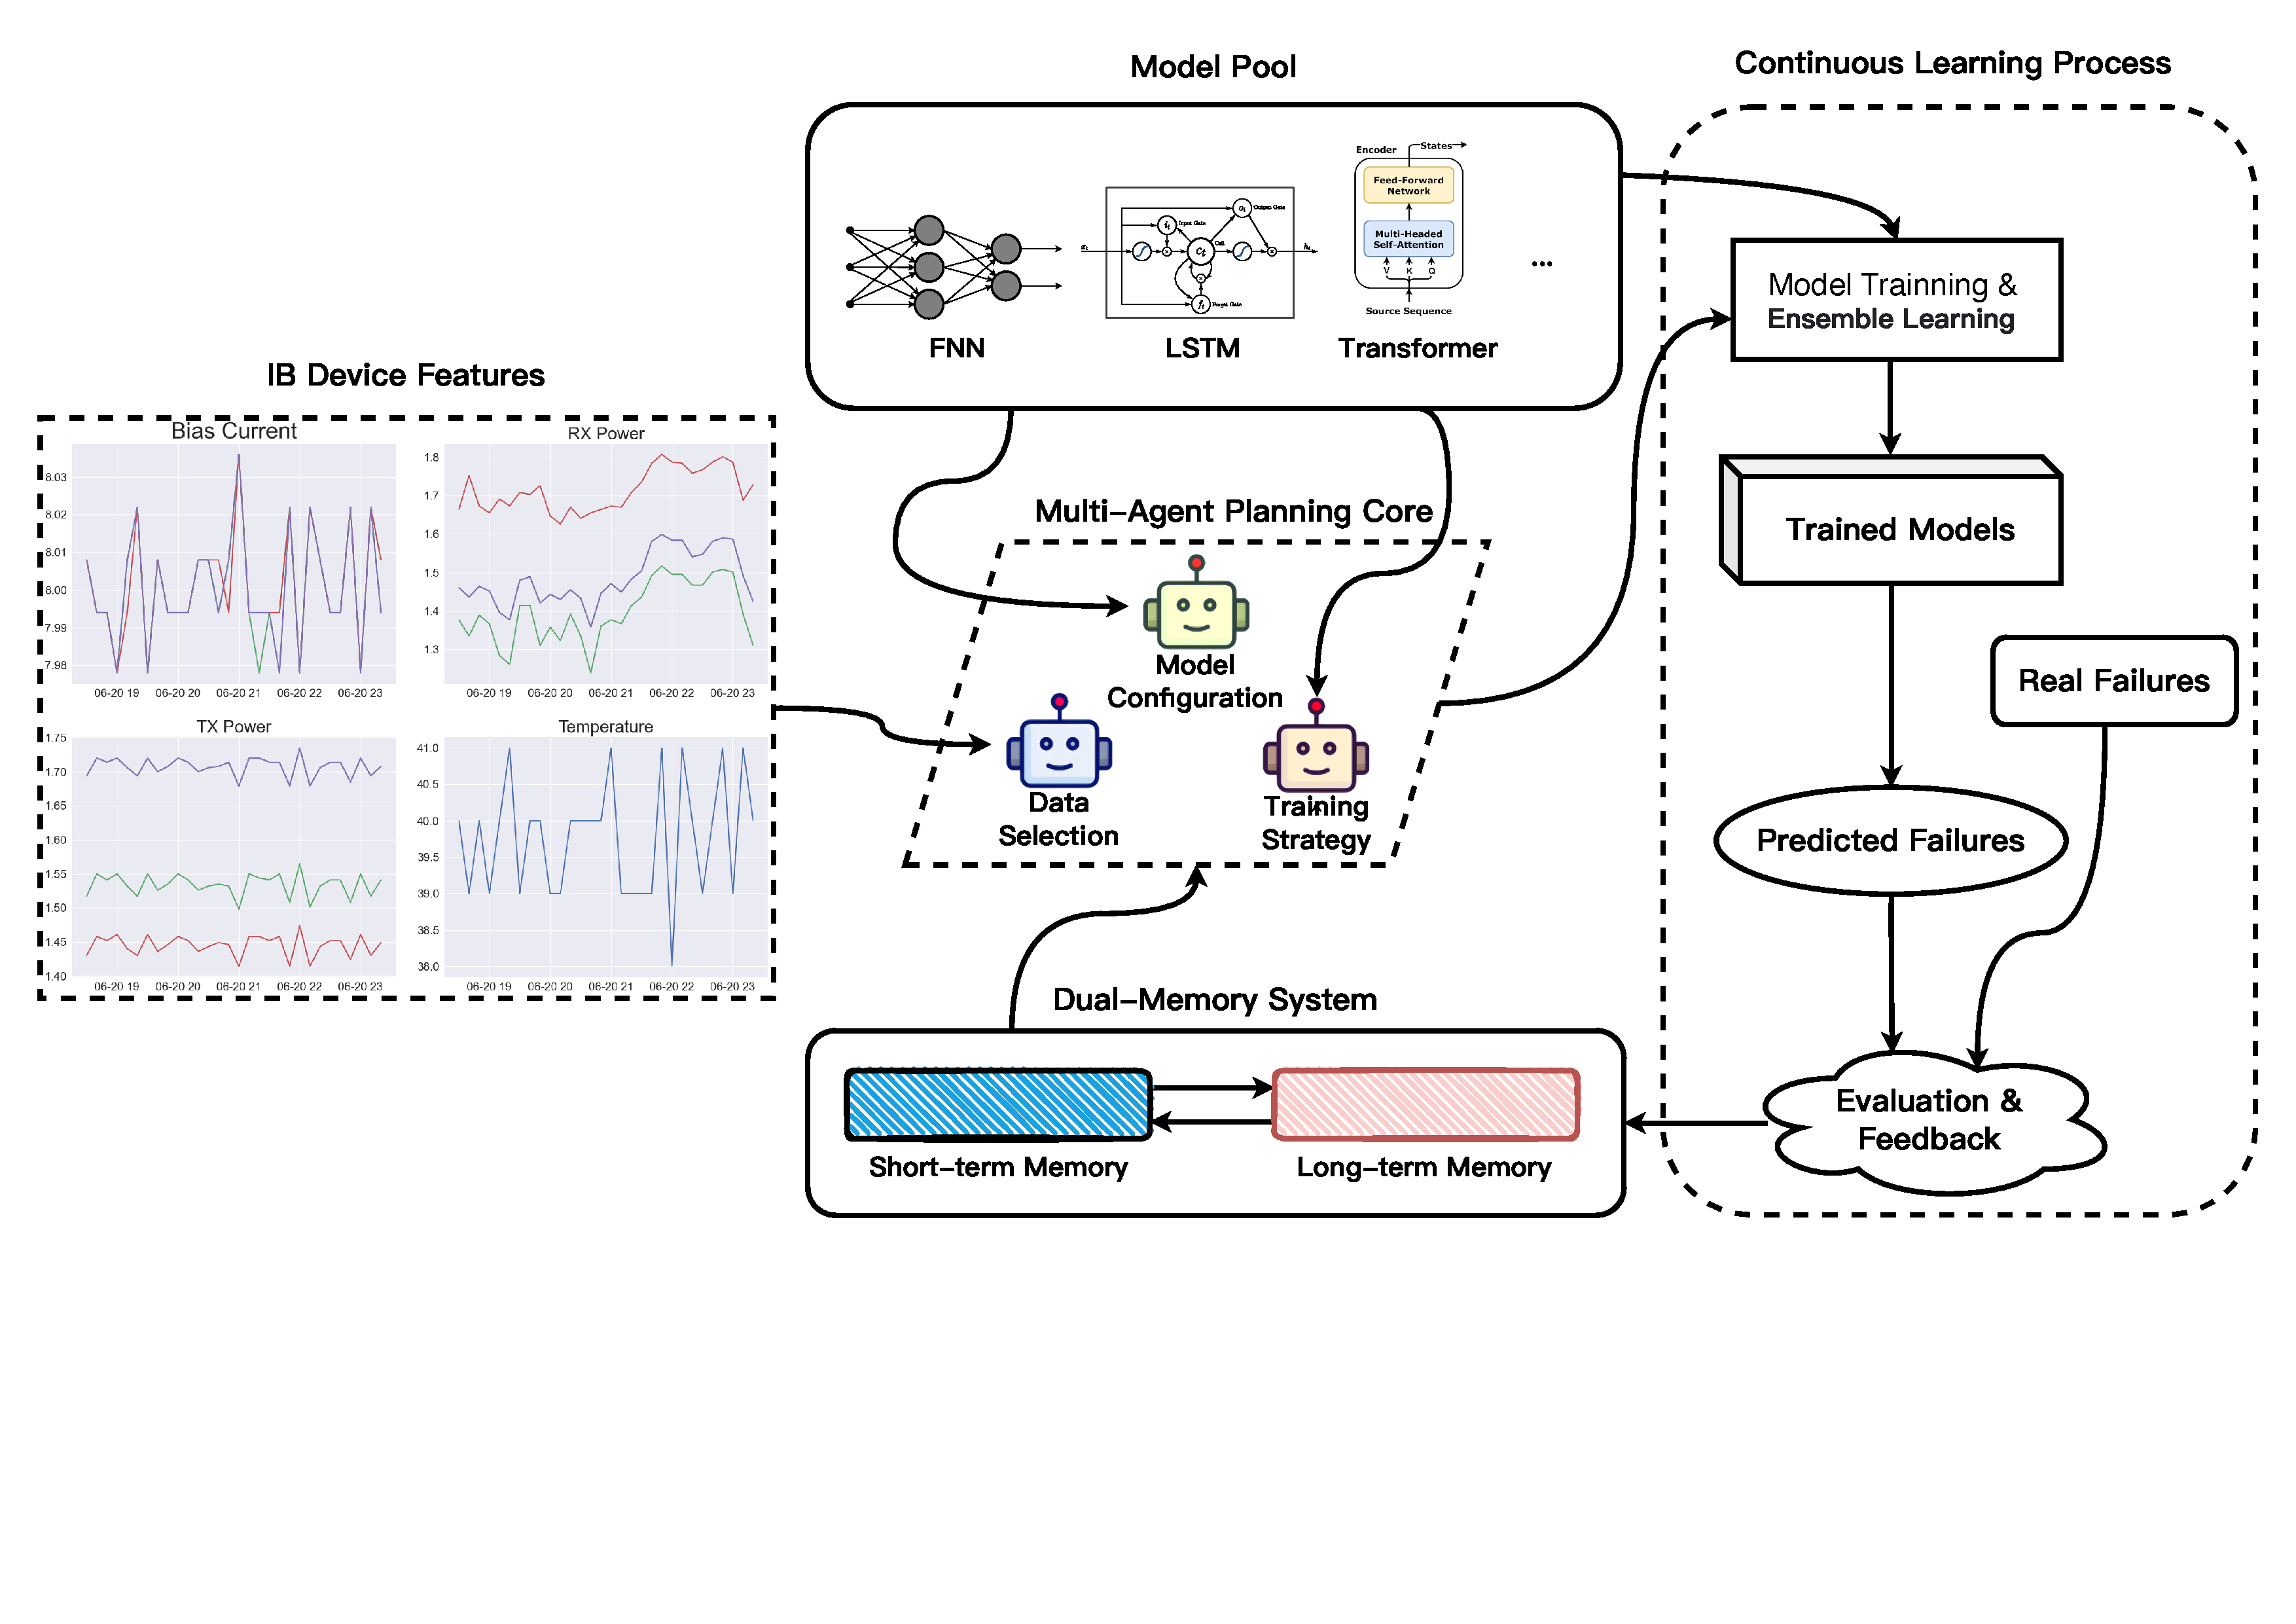
\includegraphics[width=0.95\textwidth]{fig/agent.pdf}
    \caption{Overview of SALCA-IB architecture. The system integrates (a) a model pool containing diverse deep learning models, (b) a multi-agent planning core for intelligent orchestration, (c) a dual-memory system for knowledge retention, and (d) a continuous learning process for adaptive optimization.}
    \label{fig:salca-ib}
\end{figure*}


\section{Related Work}

\subsection{IB Network Failure Prediction}

Network failure prediction, particularly in IB networks, has been extensively studied due to its critical importance in maintaining system reliability. Traditional approaches primarily rely on statistical methods and machine learning models. XXX proposed a statistical analysis framework for predicting network failures based on historical performance metrics. XXX developed a deep learning approach using LSTM networks to capture temporal dependencies in network behavior patterns. However, these methods often struggle with the inherent data scarcity in failure scenarios and lack adaptability to changing network conditions.
	
More recent work has attempted to address these challenges through ensemble methods and transfer learning. XXX introduced a multi-model ensemble approach to improve prediction robustness under limited data conditions. XXX explored transfer learning techniques to leverage knowledge from similar network environments. Despite these advances, existing methods still face significant challenges in handling dynamic network environments and maintaining long-term prediction accuracy.

\subsection{LLM in System Planning and Optimization}

The application of Large Language Models (LLMs) in system planning and optimization represents an emerging research direction. XXX demonstrated LLM's capability in generating optimization strategies for complex systems, while XXX explored using LLMs for automated system configuration and parameter tuning. These studies highlight LLM's potential in understanding system behaviors and generating sophisticated planning strategies.

In the context of network systems, XXX pioneered the use of LLMs for network management and optimization. XXX further showed how LLMs can be effectively combined with traditional machine learning models to enhance system performance. However, the application of LLMs specifically for network failure prediction remains largely unexplored, particularly in terms of continuous learning and adaptation.

\subsection{Memory-Augmented Learning Systems}

Memory mechanisms have proven crucial for enhancing learning systems' long-term performance and adaptability. XXX introduced a dual-memory architecture that separates short-term and long-term memory components, enabling both rapid adaptation and stable long-term learning. XXX developed a memory-augmented neural network that demonstrates superior performance in dynamic environments.

Recent advances in memory systems have focused on efficient memory retrieval and utilization. XXX proposed an attention-based memory access mechanism that improves memory utilization efficiency. XXX developed a hierarchical memory structure that enables more effective knowledge transfer across different tasks. These works provide valuable insights for designing memory systems, though their application in network failure prediction contexts remains limited.

\subsection{Continuous Learning for Network Systems}

Continuous learning in network systems presents unique challenges due to evolving network conditions and changing failure patterns. XXX proposed an online learning framework that continuously updates prediction models based on new observations. XXX developed an adaptive learning system that automatically adjusts to network feature distribution changes.

Recent work has increasingly focused on handling concept drift in network environments. XXX introduced a drift detection mechanism that triggers model updates when significant changes are detected. XXX proposed a sliding window approach that maintains prediction accuracy under varying network conditions. While these methods show promise, they often lack the sophisticated planning capabilities needed for complex network environments.

Unlike previous work, our SALCA-IB system uniquely combines LLM-driven planning with a dual-memory architecture, enabling both intelligent strategy generation and effective knowledge retention. This novel approach addresses the limitations of existing methods while providing superior adaptability and prediction accuracy in dynamic IB network environments.

%III. METHODOLOGY

%A. System Overview
%- SALCA-IB的整体架构图和各模块关系
%- 系统工作流程概述
%- 各核心组件的功能简介
%
%B. LLM-Driven Planning Core
%- LLM在系统中的核心规划职责
%- 训练数据选择制 (对应算法第1行)
%- 模型和参数选择策略 (对应算法第2行)
%- 反馈生成机制 (对应算法第9行)
%
%C. Dual-Memory System
%- 短期记忆和长期记忆的设计原理
%- 短期记忆更新机 (对应算法第10行)
%- 长期记忆更新机制 (对应算法第11行)
%- 记忆检索和利用策略
%
%D. Continuous Learning and Optimization
%- 在线学习机制 (对应算法第13行)
%- 性能评估方法 (对应算法第14-16行)
%- 自适应优化策略 (对应算法第12行)
%- 终止条件设计 (对应���法的while循环条件)
%
%E. Model Integration and Deployment
%- 多模型集成策略
%- 实时预测流程
%- 系统部署考虑
%- 可扩展性设计


\section{SALCA-IB}

SALCA-IB is designed as a self-adaptive intelligent system that leverages large language models (LLMs) to orchestrate network failure prediction in industrial blockchain environments. As illustrated in Fig. \ref{fig:salca-ib}, the system integrates four key components: an LLM-driven planning core, a dual-memory system, a deep learning model pool, and a continuous learning process.

As shown in Algorithm \ref{alg:salca-ib}, the LLM planning core serves as the system's central intelligence, orchestrating model selection, data processing, and strategy optimization. The dual-memory system combines short-term memory for rapid response and long-term memory for knowledge retention, enabling both immediate adaptation and sustained optimization. The model pool comprises diverse deep learning models (FNN, LSTM, and Transformer) that serve as the execution layer for failure prediction. Through continuous learning, the system evaluates prediction outcomes and adjusts strategies dynamically, ensuring robust performance in evolving network conditions. The detailed design of each component is elaborated in the following sections.

\subsection{LLM-Driven Planning Core}
Traditional failure prediction systems often rely on static model architectures and fixed training strategies, limiting their effectiveness in dynamic IB environments. Our LLM-driven planning core addresses this challenge by orchestrating three key components: data selection, model configuration, and training strategy optimization, as shown in Fig. \ref{fig:salca-ib}.

\subsubsection{Data Selection}
The data selection module intelligently processes IB network data by leveraging historical knowledge stored in long-term memory. Given the network data $\mathcal{D}$ and memory state $Mem_{long}$, the LLM performs knowledge-driven selection:
\begin{equation}
    D_{train} = \mathcal{LLM}_{select}(\mathcal{D}, Mem_{long})
\end{equation}

The selection process involves three critical aspects:

\textit{a) Temporal Window Selection}: Unlike traditional approaches that use fixed time windows, our system dynamically determines optimal training periods. This is crucial for IB networks where data patterns can be affected by external factors (e.g., network upgrades, environmental changes). The LLM analyzes historical performance patterns to identify periods with stable and representative network behavior:
\begin{equation}
    T_{window} = \arg\max_T Q_{stability}(T, Mem_{long})
\end{equation}

\textit{b) Feature Normalization}: We employ adaptive normalization strategies based on data characteristics:
\begin{equation}
    x_{norm} = \frac{x - \mu(T_{window})}{\sigma(T_{window})}
\end{equation}
where $\mu(T_{window})$ and $\sigma(T_{window})$ are calculated within the selected temporal window to avoid potential distribution shifts.

\textit{c) Sample Quality Assessment}: The LLM agent evaluates data quality by analyzing both historical patterns and current network states:
\begin{equation}
    Q(D_{train}) = \mathcal{LLM}(D_{train}, Mem_{long}, T_{window})
\end{equation}
where the LLM agent considers multiple factors including data balance, temporal correlation, and reliability based on accumulated knowledge in $Mem_{long}$. This knowledge-driven assessment enables more flexible and context-aware data selection compared to traditional weighted scoring methods.

\subsubsection{Model Configuration}
The model configuration module dynamically selects and configures models based on both current requirements and historical performance. Given the model pool $\mathcal{M}$ and memory state $Mem_{long}$, the LLM performs configuration:
\begin{equation}
    (M_{set}, \theta, S) = \mathcal{LLM}_{config}(\mathcal{M}, Mem_{long})
\end{equation}

The configuration process involves three aspects:

\textit{a) Model Selection}: The LLM selects appropriate models based on historical performance patterns and current network conditions. For example, LSTM models might be preferred for scenarios with strong temporal dependencies, while Transformers could be favored when long-range patterns are critical:
\begin{equation}
    M_{set} = \mathcal{LLM}_{select}(\mathcal{M}, Mem_{long})
\end{equation}

\textit{b) Parameter Configuration}: Instead of traditional hyperparameter optimization, the LLM leverages historical experience to directly configure model parameters:
\begin{equation}
    \theta = \mathcal{LLM}_{config}(M_{set}, Mem_{long})
\end{equation}

\textit{c) Integration Strategy}: The LLM determines the optimal ensemble strategy based on selected models' characteristics:
\begin{equation}
    M_{ensemble} = TrainEnsemble(M_{set}, \theta, S, D_{train})
\end{equation}

\subsubsection{Training Strategy}
The training strategy module optimizes the learning process through LLM-driven decisions. The optimization process considers:

\textit{a) Performance Evaluation}: The LLM evaluates current model performance:
\begin{equation}
    E = Evaluate(P_{failures}, R_{failures})
\end{equation}

\textit{b) Feedback Generation}: Based on evaluation results, the LLM generates optimization feedback:
\begin{equation}
    F = \mathcal{LLM}_{feedback}(E, M_{ensemble}, \theta, S)
\end{equation}

\textit{c) Model Update}: The ensemble model is continuously updated based on the feedback:
\begin{equation}
    M_{ensemble} = UpdateEnsemble(M_{set}, \theta, S, D_{new})
\end{equation}

Through these mechanisms, our system achieves dynamic model selection and training optimization, leveraging both historical knowledge and current network states for improved prediction performance.

\subsection{Dual-Memory System}
Traditional single-memory approaches often struggle to balance immediate adaptability with long-term knowledge retention in dynamic network environments. Moreover, directly feeding extensive historical data to LLMs can lead to context overflow and degraded planning performance. To address these limitations, we propose a dual-memory system that enables both efficient LLM-based decision making and effective knowledge preservation.

\subsubsection{Memory Architecture}
The dual-memory system consists of two complementary components: short-term memory $Mem_{short}$ and long-term memory $Mem_{long}$. This separation serves two key purposes: (1) enabling rapid response through focused recent information, and (2) managing LLM's context length limitation through structured historical knowledge representation.

\textit{a) Short-term Memory Structure}: The short-term memory maintains recent operational states and decisions. For operational efficiency, it stores current feature set $F_{set}$ with selection rationale, time window configurations $T_{window}$, and model performance metrics $P_{model}$ including accuracy, precision, recall and F1-score. Additionally, it records current model configurations $M_{config}$ with ensemble strategies and data characteristics $D_{char}$ for rapid access. The short-term memory is formalized as:
\begin{equation}
    Mem_{short} = \{(F_{set}, T_{window}, P_{model}, M_{config}, D_{char})\}
\end{equation}

\textit{b) Long-term Memory Structure}: The long-term memory preserves historical knowledge and patterns essential for sustained performance. It maintains comprehensive feature statistics $F_{stats}$ including temporal distributions and correlations, historical time step patterns $T_{step}$, and feature selection patterns $F_{patterns}$ across different operational periods. The long-term memory is formalized as:
\begin{equation}
    Mem_{long} = \{(F_{list}, T_{step}, F_{stats}, F_{patterns})\}
\end{equation}

\subsubsection{Memory Interaction Mechanism}
The dual-memory system maintains bidirectional knowledge flow through two distinct interaction paths:

\textit{a) Short-term to Long-term Transfer}: The system continuously evaluates and transfers valuable information from short-term to long-term memory:
\begin{equation}
    Mem_{long} = UpdatePatterns(Mem_{long}, Mem_{short})
\end{equation}
This process includes updating feature selection patterns based on successful predictions, refining model configuration strategies that yield high performance, and accumulating effective time window selections. The transfer mechanism employs significance filtering to ensure only valuable patterns are preserved:
\begin{equation}
    Significance = \mathcal{LLM}(P_{model}, F_{patterns}, T_{window})
\end{equation}

\textit{b) Long-term to Short-term Reference}: When making current decisions, the system retrieves relevant historical knowledge from long-term memory to guide short-term operations:
\begin{equation}
    Knowledge = RetrievePatterns(Mem_{long}, State_{current})
\end{equation}
This retrieved knowledge assists in feature selection, model configuration, and training strategy optimization. The LLM then combines this historical knowledge with current states for decision making:
\begin{equation}
    Decision = \mathcal{LLM}(State_{current}, Knowledge, Mem_{short})
\end{equation}

Through this bidirectional interaction mechanism, SALCA-IB achieves both knowledge preservation and efficient utilization. The short-term to long-term transfer ensures continuous learning and pattern accumulation, while the long-term to short-term reference enables experience-driven decision making without overwhelming the LLM's context capacity.

\subsection{Continuous Learning and Optimization}
Traditional static prediction models often fail to maintain performance as network conditions evolve. SALCA-IB addresses this challenge through a comprehensive continuous learning framework that combines online model updates with LLM-driven optimization strategies.

\begin{algorithm}[t]
    \caption{SALCA-IB}
    \label{alg:salca-ib}
    \begin{algorithmic}[1]
    \Require
        \Statex \hspace{-1em}Network data $\mathcal{D}$, Large language model $\mathcal{L}$
        \Statex \hspace{-1em}Model pool $\mathcal{M} = \{FNN, LSTM, Transformer\}$
        \Statex \hspace{-1em}Dual-memory system: $Mem_{short}$, $Mem_{long}$
        \Statex \hspace{-1em}Parameters: $T_{max}$ (max iterations), $\delta$ (convergence threshold)
    
    \vspace{0.5em}
    \State $D_{train} = \mathcal{LLM}_{select}(\mathcal{D}, Mem_{long})$ \Comment{Knowledge-driven selection}
    
    \State $(M_{set}, \theta, S) = \mathcal{LLM}_{config}(\mathcal{M}, Mem_{long})$ \Comment{Model configuration}
    
    \State $M_{ensemble} = TrainEnsemble(M_{set}, \theta, S, D_{train})$ \Comment{Initialize ensemble}
    
    \State $perf_{prev} = Evaluate(M_{ensemble}, D_{val})$ \Comment{Baseline evaluation}
    
    \State $t = 0$
    
    \While{$t < T_{max}$ \textbf{and} $\Delta_{perf} > \delta$}
        \State $P_{failures} = Predict(M_{ensemble}, D_{new})$ \Comment{Failure prediction}
        
        \State $R_{failures} = CollectReal(D_{actual})$ \Comment{Ground truth}
        
        \State $E = Evaluate(P_{failures}, R_{failures})$ \Comment{Assessment}
        
        \State $F = \mathcal{LLM}_{feedback}(E, M_{ensemble}, \theta, S)$ \Comment{Generate feedback}
        
        \State $Mem_{short}.update(P_{failures}, R_{failures}, F)$ \Comment{Update short-term}
        
        \State $Mem_{long}.update(F, M_{ensemble}, \theta, S)$ \Comment{Update long-term}
        
        \State $(M_{set}, \theta, S, D_{train}) = \mathcal{LLM}_{optimize}(Mem_{short}, Mem_{long})$ \Comment{Optimize}
        
        \State $M_{ensemble}.update(M_{set}, \theta, S, D_{new})$ \Comment{Continuous learning}
        
        \State $perf_{current} = Evaluate(M_{ensemble}, D_{val})$     
        \State $\Delta_{perf} = perf_{current} - perf_{prev}$
        \State $perf_{prev} = perf_{current}$
        \State $t = t + 1$
    \EndWhile
    
    \State \Return $M_{ensemble}, \theta, S, Mem_{short}, Mem_{long}$ 
    \end{algorithmic}
    \end{algorithm}
    

\subsubsection{Continuous Assessment Process}
The system performs continuous assessment of prediction performance through failure prediction ($P_{failures}$), reality collection ($R_{failures}$), and evaluation ($E$):
\begin{equation}
    E = Evaluate(P_{failures}, R_{failures})
\end{equation}

\subsubsection{LLM-Driven Feedback Generation}
The feedback generation process forms the core of our self-refinement mechanism:

\textit{a) Structured Feedback Generation}: The LLM analyzes performance metrics and generates specific, actionable feedback. This structured feedback encompasses architectural refinements for model components, feature importance adjustments, training strategy optimization, and ensemble weight recalibration. The generation process is formalized as:
\begin{equation}
    F = \mathcal{LLM}_{feedback}(E, M_{ensemble}, \theta, S)
\end{equation}

\textit{b) Memory Integration}: The system integrates feedback into its dual-memory architecture. Short-term memory captures recent feedback patterns and their immediate effects, while long-term memory preserves effective optimization strategies and their associated performance improvements:
\begin{equation}
    Mem_{short}.update(P_{failures}, R_{failures}, F)
\end{equation}
\begin{equation}
    Mem_{long}.update(F, M_{ensemble}, \theta, S)
\end{equation}

\subsubsection{Feedback-Driven Model Update}
The system implements feedback through a structured update process:

\textit{a) Configuration Optimization}: The LLM leverages feedback and memory states to optimize model configurations, ensuring that updates align with both recent performance patterns and long-term optimization strategies:
\begin{equation}
    (M_{set}, \theta, S, D_{train}) = \mathcal{LLM}_{optimize}(Mem_{short}, Mem_{long})
\end{equation}

\textit{b) Model Update}: The ensemble model is updated based on the optimized configuration and new data:
\begin{equation}
    M_{ensemble} = UpdateEnsemble(M_{set}, \theta, S, D_{new})
\end{equation}

Through this feedback-centric learning framework, SALCA-IB achieves true self-refinement capability. The system not only adapts to changing conditions but also accumulates effective optimization strategies through LLM-generated feedback, enabling continuous performance improvement while maintaining operational stability.



\section{Experimental Evaluation}

\subsection{Experimental Setup}
% - IB网络数据集描述(来源、规模、特征分布等)
% - 评估指标定义(准确率、F1-score、预测延迟等)
% - 基线方法介绍(传统ML方法、现有故障预测系统等)
% - 实验环境配置(硬件、软件环境)
% - SALCA-IB参数设置(记忆容量、更新阈值等)

\subsection{Overall Performance Comparison}
% - 与基线方法的全面对比
% - 不同评估指标下的性能分析
% - 在不同网络条件下的表现比较
% - 统计显著性分析

\subsection{Adaptability Analysis}
% - 网络特征分布变化场景下的性能评估
% - 模型适应速度分析
% - 预测稳定性研究
% - 与现有自适应方法的对比

\subsection{Ablation Study}
% - LLM规划核心的贡献分析
% - 双重记忆系统的效果验证
% - 在线学习机制的重要性
% - 各个创新组件的独立贡献评估

\subsection{Case Study}
% - 典型故障预测案例分析
% - LLM决策过程的可解释性展示
% - 记忆系统工作机制的实例说明
% - 系统适应过程的可视化

\subsection{Efficiency and Overhead Analysis}
% - 计算资源消耗评估
% - 内存使用效率分析
% - 预测延迟分析
% - 系统扩展性研究

\section{Ease of Use}

\subsection{Maintaining the Integrity of the Specifications}

The IEEEtran class file is used to format your paper and style the text. All margins, 
column widths, line spaces, and text fonts are prescribed; please do not 
alter them. You may note peculiarities. For example, the head margin
measures proportionately more than is customary. This measurement 
and others are deliberate, using specifications that anticipate your paper 
as one part of the entire proceedings, and not as an independent document. 
Please do not revise any of the current designations.

\section{Prepare Your Paper Before Styling}
Before you begin to format your paper, first write and save the content as a 
separate text file. Complete all content and organizational editing before 
formatting. Please note sections \ref{AA}--\ref{SCM} below for more information on 
proofreading, spelling and grammar.

Keep your text and graphic files separate until after the text has been 
formatted and styled. Do not number text heads---{\LaTeX} will do that 
for you.

\subsection{Abbreviations and Acronyms}\label{AA}
Define abbreviations and acronyms the first time they are used in the text, 
even after they have been defined in the abstract. Abbreviations such as 
IEEE, SI, MKS, CGS, ac, dc, and rms do not have to be defined. Do not use 
abbreviations in the title or heads unless they are unavoidable.

\subsection{Units}
\begin{itemize}
\item Use either SI (MKS) or CGS as primary units. (SI units are encouraged.) English units may be used as secondary units (in parentheses). An exception would be the use of English units as identifiers in trade, such as ``3.5-inch disk drive''.
\item Avoid combining SI and CGS units, such as current in amperes and magnetic field in oersteds. This often leads to confusion because equations do not balance dimensionally. If you must use mixed units, clearly state the units for each quantity that you use in an equation.
\item Do not mix complete spellings and abbreviations of units: ``Wb/m\textsuperscript{2}'' or ``webers per square meter'', not ``webers/m\textsuperscript{2}''. Spell out units when they appear in text: ``. . . a few henries'', not ``. . . a few H''.
\item Use a zero before decimal points: ``0.25'', not ``.25''. Use ``cm\textsuperscript{3}'', not ``cc''.)
\end{itemize}

\subsection{Equations}
Number equations consecutively. To make your 
equations more compact, you may use the solidus (~/~), the exp function, or 
appropriate exponents. Italicize Roman symbols for quantities and variables, 
but not Greek symbols. Use a long dash rather than a hyphen for a minus 
sign. Punctuate equations with commas or periods when they are part of a 
sentence, as in:
\begin{equation}
a+b=\gamma\label{eq}
\end{equation}

Be sure that the 
symbols in your equation have been defined before or immediately following 
the equation. Use ``\eqref{eq}'', not ``Eq.~\eqref{eq}'' or ``equation \eqref{eq}'', except at 
the beginning of a sentence: ``Equation \eqref{eq} is . . .''

\subsection{\LaTeX-Specific Advice}

Please use ``soft'' (e.g., \verb|\eqref{Eq}|) cross references instead
of ``hard'' references (e.g., \verb|(1)|). That will make it possible
to combine sections, add equations, or change the order of figures or
citations without having to go through the file line by line.

Please don't use the \verb|{eqnarray}| equation environment. Use
\verb|{align}| or \verb|{IEEEeqnarray}| instead. The \verb|{eqnarray}|
environment leaves unsightly spaces around relation symbols.

Please note that the \verb|{subequations}| environment in {\LaTeX}
will increment the main equation counter even when there are no
equation numbers displayed. If you forget that, you might write an
article in which the equation numbers skip from (17) to (20), causing
the copy editors to wonder if you've discovered a new method of
counting.

{\BibTeX} does not work by magic. It doesn't get the bibliographic
data from thin air but from .bib files. If you use {\BibTeX} to produce a
bibliography you must send the .bib files. 

{\LaTeX} can't read your mind. If you assign the same label to a
subsubsection and a table, you might find that Table I has been cross
referenced as Table IV-B3. 

{\LaTeX} does not have precognitive abilities. If you put a
\verb|\label| command before the command that updates the counter it's
supposed to be using, the label will pick up the last counter to be
cross referenced instead. In particular, a \verb|\label| command
should not go before the caption of a figure or a table.

Do not use \verb|\nonumber| inside the \verb|{array}| environment. It
will not stop equation numbers inside \verb|{array}| (there won't be
any anyway) and it might stop a wanted equation number in the
surrounding equation.

\subsection{Some Common Mistakes}\label{SCM}
\begin{itemize}
\item The word ``data'' is plural, not singular.
\item The subscript for the permeability of vacuum $\mu_{0}$, and other common scientific constants, is zero with subscript formatting, not a lowercase letter ``o''.
\item In American English, commas, semicolons, periods, question and exclamation marks are located within quotation marks only when a complete thought or name is cited, such as a title or full quotation. When quotation marks are used, instead of a bold or italic typeface, to highlight a word or phrase, punctuation should appear outside of the quotation marks. A parenthetical phrase or statement at the end of a sentence is punctuated outside of the closing parenthesis (like this). (A parenthetical sentence is punctuated within the parentheses.)
\item A graph within a graph is an ``inset'', not an ``insert''. The word alternatively is preferred to the word ``alternately'' (unless you really mean something that alternates).
\item Do not use the word ``essentially'' to mean ``approximately'' or ``effectively''.
\item In your paper title, if the words ``that uses'' can accurately replace the word ``using'', capitalize the ``u''; if not, keep using lower-cased.
\item Be aware of the different meanings of the homophones ``affect'' and ``effect'', ``complement'' and ``compliment'', ``discreet'' and ``discrete'', ``principal'' and ``principle''.
\item Do not confuse ``imply'' and ``infer''.
\item The prefix ``non'' is not a word; it should be joined to the word it modifies, usually without a hyphen.
\item There is no period after the ``et'' in the Latin abbreviation ``et al.''.
\item The abbreviation ``i.e.'' means ``that is'', and the abbreviation ``e.g.'' means ``for example''.
\end{itemize}
An excellent style manual for science writers is \cite{b7}.

\subsection{Authors and Affiliations}
\textbf{The class file is designed for, but not limited to, six authors.} A 
minimum of one author is required for all conference articles. Author names 
should be listed starting from left to right and then moving down to the 
next line. This is the author sequence that will be used in future citations 
and by indexing services. Names should not be listed in columns nor group by 
affiliation. Please keep your affiliations as succinct as possible (for 
example, do not differentiate among departments of the same organization).

\subsection{Identify the Headings}
Headings, or heads, are organizational devices that guide the reader through 
your paper. There are two types: component heads and text heads.

Component heads identify the different components of your paper and are not 
topically subordinate to each other. Examples include Acknowledgments and 
References and, for these, the correct style to use is ``Heading 5''. Use 
``figure caption'' for your Figure captions, and ``table head'' for your 
table title. Run-in heads, such as ``Abstract'', will require you to apply a 
style (in this case, italic) in addition to the style provided by the drop 
down menu to differentiate the head from the text.

Text heads organize the topics on a relational, hierarchical basis. For 
example, the paper title is the primary text head because all subsequent 
material relates and elaborates on this one topic. If there are two or more 
sub-topics, the next level head (uppercase Roman numerals) should be used 
and, conversely, if there are not at least two sub-topics, then no subheads 
should be introduced.

\subsection{Figures and Tables}
\paragraph{Positioning Figures and Tables} Place figures and tables at the top and 
bottom of columns. Avoid placing them in the middle of columns. Large 
figures and tables may span across both columns. Figure captions should be 
below the figures; table heads should appear above the tables. Insert 
figures and tables after they are cited in the text. Use the abbreviation 
``Fig.~\ref{fig}'', even at the beginning of a sentence.

\begin{table}[htbp]
\caption{Table Type Styles}
\begin{center}
\begin{tabular}{|c|c|c|c|}
\hline
\textbf{Table}&\multicolumn{3}{|c|}{\textbf{Table Column Head}} \\
\cline{2-4} 
\textbf{Head} & \textbf{\textit{Table column subhead}}& \textbf{\textit{Subhead}}& \textbf{\textit{Subhead}} \\
\hline
copy& More table copy$^{\mathrm{a}}$& &  \\
\hline
\multicolumn{4}{l}{$^{\mathrm{a}}$Sample of a Table footnote.}
\end{tabular}
\label{tab1}
\end{center}
\end{table}


Figure Labels: Use 8 point Times New Roman for Figure labels. Use words 
rather than symbols or abbreviations when writing Figure axis labels to 
avoid confusing the reader. As an example, write the quantity 
``Magnetization'', or ``Magnetization, M'', not just ``M''. If including 
units in the label, present them within parentheses. Do not label axes only 
with units. In the example, write ``Magnetization (A/m)'' or ``Magnetization 
\{A[m(1)]\}'', not just ``A/m''. Do not label axes with a ratio of 
quantities and units. For example, write ``Temperature (K)'', not 
``Temperature/K''.

\section*{Acknowledgment}

The preferred spelling of the word ``acknowledgment'' in America is without 
an ``e'' after the ``g''. Avoid the stilted expression ``one of us (R. B. 
G.) thanks $\ldots$''. Instead, try ``R. B. G. thanks$\ldots$''. Put sponsor 
acknowledgments in the unnumbered footnote on the first page.

\section*{References}

Please number citations consecutively within brackets \cite{b1}. The 
sentence punctuation follows the bracket \cite{b2}. Refer simply to the reference 
number, as in \cite{b3}---do not use ``Ref. \cite{b3}'' or ``reference \cite{b3}'' except at 
the beginning of a sentence: ``Reference \cite{b3} was the first $\ldots$''

Number footnotes separately in superscripts. Place the actual footnote at 
the bottom of the column in which it was cited. Do not put footnotes in the 
abstract or reference list. Use letters for table footnotes.

Unless there are six authors or more give all authors' names; do not use 
``et al.''. Papers that have not been published, even if they have been 
submitted for publication, should be cited as ``unpublished'' \cite{b4}. Papers 
that have been accepted for publication should be cited as ``in press'' \cite{b5}. 
Capitalize only the first word in a paper title, except for proper nouns and 
element symbols.

For papers published in translation journals, please give the English 
citation first, followed by the original foreign-language citation \cite{b6}.

\begin{thebibliography}{00}
\bibitem{b1} G. Eason, B. Noble, and I. N. Sneddon, ``On certain integrals of Lipschitz-Hankel type involving products of Bessel functions,'' Phil. Trans. Roy. Soc. London, vol. A247, pp. 529--551, April 1955.
\bibitem{b2} J. Clerk Maxwell, A Treatise on Electricity and Magnetism, 3rd ed., vol. 2. Oxford: Clarendon, 1892, pp.68--73.
\bibitem{b3} I. S. Jacobs and C. P. Bean, ``Fine particles, thin films and exchange anisotropy,'' in Magnetism, vol. III, G. T. Rado and H. Suhl, Eds. New York: Academic, 1963, pp. 271--350.
\bibitem{b4} K. Elissa, ``Title of paper if known,'' unpublished.
\bibitem{b5} R. Nicole, ``Title of paper with only first word capitalized,'' J. Name Stand. Abbrev., in press.
\bibitem{b6} Y. Yorozu, M. Hirano, K. Oka, and Y. Tagawa, ``Electron spectroscopy studies on magneto-optical media and plastic substrate interface,'' IEEE Transl. J. Magn. Japan, vol. 2, pp. 740--741, August 1987 [Digests 9th Annual Conf. Magnetics Japan, p. 301, 1982].
\bibitem{b7} M. Young, The Technical Writer's Handbook. Mill Valley, CA: University Science, 1989.
\end{thebibliography}
\vspace{12pt}
\color{red}
IEEE conference templates contain guidance text for composing and formatting conference papers. Please ensure that all template text is removed from your conference paper prior to submission to the conference. Failure to remove the template text from your paper may result in your paper not being published.

\end{document}
